\documentclass[aspectratio=169]{beamer}
\usetheme{metropolis}

\usepackage[utf8]{inputenc}
\usepackage[english]{babel}
\usepackage{amsmath}
\usepackage{amsfonts}
\usepackage{booktabs}
\usepackage{listings}
\usepackage{subcaption}
\usepackage{tikz}
\usepackage{pgfplots}
\pgfplotsset{compat=1.16}
\usetikzlibrary{positioning, arrows.meta, fit, calc, shapes.misc, backgrounds}

% Configuración para bloques de código Python
\lstset{
	language=Python,
	basicstyle=\ttfamily\scriptsize,
	keywordstyle=\color{blue},
	commentstyle=\color{green!50!black},
	stringstyle=\color{orange},
	breaklines=true,
	frame=single,
	showstringspaces=false
}

% Estilos TikZ reutilizables
\tikzset{
	box/.style={draw, rounded corners=3pt, minimum width=3.2cm, minimum height=0.55cm, font=\scriptsize, align=center, fill=white},
	dbox/.style={box, fill=gray!70, text=white},
	fbox/.style={box, fill=gray!25},
	arr/.style={-{Stealth[length=2mm]}, thick},
	done/.style={box, fill=green!15, draw=green!50!black},
	todo/.style={box, minimum width=2.3cm}
}

\title{LLMs \& VLMs course}
\subtitle{Implementing a GPT model from scratch}
\author{Juan Irving Vasquez}
\date{\today}
\institute{Instituto Politécnico Nacional (IPN)}
\titlegraphic{
\includegraphics[height=1.2cm]{ipn-cidetec.png}\hspace{0.1cm}
\includegraphics[height=1.2cm]{escudoESCOM}}

% Tokens para la diapositiva de generación
\newcommand{\tk}[1]{\tikz[baseline=(t.base)]\node[draw, rounded corners=2pt, fill=blue!10, font=\ttfamily\scriptsize, inner sep=2pt](t){\strut #1};}
\newcommand{\nw}[1]{\tikz[baseline=(t.base)]\node[draw, rounded corners=2pt, fill=red!15, dashed, thick, font=\ttfamily\scriptsize, inner sep=2pt](t){\strut #1};}

% Mapa mental del capítulo: #1 = número de bloques completados (0-7)
\newcommand{\roadmapfig}[1]{%
	\begin{tikzpicture}[node distance=0.35cm and 0.25cm]
		\node[todo] (b2) {2) Layer\\normalization};
		\node[todo, right=of b2] (b3) {3) GELU\\activation};
		\node[todo, right=of b3] (b4) {4) Feed forward\\network};
		\node[todo, right=of b4] (b5) {5) Shortcut\\connections};
		\node[todo, above=0.9cm of $(b3)!0.5!(b4)$] (b6) {6) Transformer\\block};
		\node[todo, above=0.5cm of b6] (b7) {7) Final GPT\\architecture};
		\node[todo, below=0.5cm of $(b3)!0.5!(b4)$] (b1) {1) GPT\\backbone};
		\foreach \n in {2,3,4,5} \draw[arr] (b\n.north) -- (b6.south);
		\draw[arr] (b6) -- (b7);
		\foreach \n/\t in {1/{1) GPT\\backbone},2/{2) Layer\\normalization},3/{3) GELU\\activation},4/{4) Feed forward\\network},5/{5) Shortcut\\connections},6/{6) Transformer\\block},7/{7) Final GPT\\architecture}} {
			\ifnum\n<#1\relax \node[done, minimum width=2.3cm] at (b\n) {\t}; \node[text=green!50!black, font=\large] at (b\n.north east) {$\checkmark$}; \fi
		}
	\end{tikzpicture}%
}

\begin{document}
	
	\maketitle
	
	\frame{
		\frametitle{Contents}
		\tableofcontents
	}
	
	\AtBeginSection[] { \begin{frame} \frametitle{Roadmap} \tableofcontents[currentsection] \end{frame} }
	
	% =====================================================================
	\section{From attention to a full GPT}
	% =====================================================================
	
	\begin{frame}{Where are we?}
		\centering
		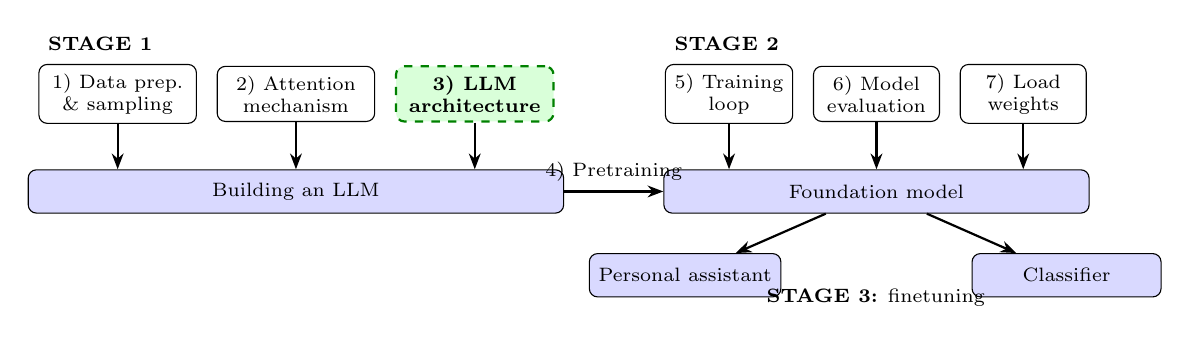
\begin{tikzpicture}[node distance=0.25cm, every node/.style={font=\scriptsize}]
			\node[box, minimum width=2cm] (s1) {1) Data prep.\\\& sampling};
			\node[box, minimum width=2cm, right=of s1] (s2) {2) Attention\\mechanism};
			\node[box, minimum width=2cm, right=of s2, fill=green!15, draw=green!50!black, thick, dashed] (s3) {\textbf{3) LLM}\\\textbf{architecture}};
			\node[box, minimum width=6.8cm, below=0.6cm of s2, fill=blue!15] (build) {Building an LLM};
			\foreach \n in {s1,s2,s3} \draw[arr] (\n.south) -- (\n.south |- build.north);
			\node[above=0.05cm of s1.north west, anchor=south west] {\textbf{STAGE 1}};
			
			\node[box, minimum width=1.6cm, right=1.4cm of s3] (s5) {5) Training\\loop};
			\node[box, minimum width=1.6cm, right=of s5] (s6) {6) Model\\evaluation};
			\node[box, minimum width=1.6cm, right=of s6] (s7) {7) Load\\weights};
			\node[box, minimum width=5.4cm, fill=blue!15] (fm) at (s6 |- build) {Foundation model};
			\foreach \n in {s5,s6,s7} \draw[arr] (\n.south) -- (\n.south |- fm.north);
			\node[above=0.05cm of s5.north west, anchor=south west] {\textbf{STAGE 2}};
			\draw[arr] (build) -- node[above]{4) Pretraining} (fm);
			
			\node[box, minimum width=2.4cm, fill=blue!15, below right=0.5cm and -1.5cm of fm] (cls) {Classifier};
			\node[box, minimum width=2.4cm, fill=blue!15, below left=0.5cm and -1.5cm of fm] (pa) {Personal assistant};
			\draw[arr] (fm) -- (cls);
			\draw[arr] (fm) -- (pa);
			\node[below=0.05cm of $(pa)!0.5!(cls)$] {\textbf{STAGE 3:} finetuning};
		\end{tikzpicture}
		
		\vspace{0.3cm}
		\small Last session: \textbf{multi-head attention}. Today: the \textbf{other building blocks} and how to assemble them into a GPT-like model.
	\end{frame}
	
	\begin{frame}{A mental model of a GPT model}
		\begin{columns}[c]
			\column{0.45\textwidth}
			\centering
			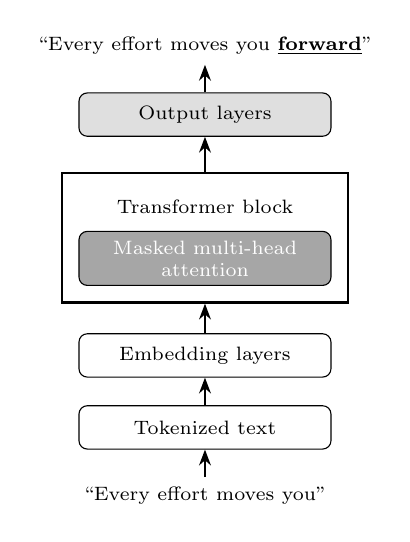
\begin{tikzpicture}[node distance=0.35cm]
				\node (in) {\scriptsize ``Every effort moves you''};
				\node[box, above=of in] (tok) {Tokenized text};
				\node[box, above=of tok] (emb) {Embedding layers};
				\node[dbox, above=0.6cm of emb] (mha) {Masked multi-head\\attention};
				\node[font=\scriptsize, above=0.1cm of mha] (tbl) {Transformer block};
				\node[draw, thick, fit=(mha)(tbl), inner sep=6pt] (tb) {};
				\node[fbox, above=0.45cm of tb] (out) {Output layers};
				\node[above=of out] (o) {\scriptsize ``Every effort moves you \textbf{\underline{forward}}''};
				\draw[arr] (in) -- (tok); \draw[arr] (tok) -- (emb); \draw[arr] (emb) -- (tb);
				\draw[arr] (tb) -- (out); \draw[arr] (out) -- (o);
			\end{tikzpicture}
			\column{0.55\textwidth}
			\begin{itemize}
				\item GPT = \textbf{G}enerative \textbf{P}retrained \textbf{T}ransformer.
				\item Generates new text \textbf{one token at a time}.
				\item Despite its size, the architecture is simple: most components are \textbf{repeated}.
				\item Today: the \textbf{transformer block} and the full model.
			\end{itemize}
		\end{columns}
	\end{frame}
	
	\begin{frame}{Target: GPT-2 \emph{small} (124M parameters)}
		\begin{columns}[T]
			\column{0.5\textwidth}
			\small
			\begin{itemize}
				\item Radford et al., \emph{Language Models are Unsupervised Multitask Learners} (2019).
				\item Weights are \textbf{publicly available} $\Rightarrow$ we can load them later.
				\item GPT-3 has the same architecture, scaled from 1.5B to \textbf{175B} parameters.
				\item GPT-2 runs on a laptop; GPT-3 would take $\sim$355 years to train on a single V100.
			\end{itemize}
			\vspace{0.2cm}
			\begin{alertblock}{Parameters}
				\footnotesize Trainable weights. A $2048\times2048$ layer already has $4{,}194{,}304$ parameters.
			\end{alertblock}
			\column{0.5\textwidth}
			\centering
			\footnotesize
			\begin{tabular}{lrr}
				\toprule
				\textbf{Model} & \textbf{Params} & \textbf{Layers} \\
				\midrule
				GPT-2 small  & 124M   & 12 \\
				GPT-2 medium & 355M   & 24 \\
				GPT-2 large  & 774M   & 36 \\
				GPT-2 XL     & 1{,}558M & 48 \\
				\midrule
				GPT-3        & 175B   & 96 \\
				\bottomrule
			\end{tabular}
		\end{columns}
	\end{frame}
	
	
	
	\begin{frame}[fragile]{The model configuration}
		\begin{columns}[T]
			\column{0.55\textwidth}
			\begin{lstlisting}[basicstyle=\ttfamily\tiny]
	GPT_CONFIG_124M = {
		"vocab_size": 50257,    # Vocabulary size
		"context_length": 1024, # Context length
		"emb_dim": 768,         # Embedding dim
		"n_heads": 12,          # Attention heads
		"n_layers": 12,         # Transformer blocks
		"drop_rate": 0.1,       # Dropout rate
		"qkv_bias": False       # Query-Key-Value bias
	}
			\end{lstlisting}
			\column{0.43\textwidth}
			\footnotesize
			\begin{itemize}
				\item \texttt{vocab\_size}: BPE tokenizer vocabulary (Ch.~2).
				\item \texttt{context\_length}: max. input tokens (positional embeddings).
				\item \texttt{emb\_dim}: each token $\to$ 768-d vector.
				\item \texttt{n\_heads}: heads in multi-head attention.
				\item \texttt{n\_layers}: number of transformer blocks.
				\item \texttt{drop\_rate}: 10\% of hidden units dropped.
				\item \texttt{qkv\_bias}: bias in $W^Q, W^K, W^V$ (off, as in modern LLMs).
			\end{itemize}
		\end{columns}
	\end{frame}
	
	\begin{frame}{Plan for this session}
		\centering
		\roadmapfig{0}
		
		\vspace{0.3cm}
		\small We start with a \textbf{placeholder backbone} to see the big picture, then fill in blocks 2--5, assemble block 6, and finish with the full GPT (7).
	\end{frame}
	
	\begin{frame}[fragile]{Step 1: A placeholder GPT backbone}
		\begin{lstlisting}[basicstyle=\ttfamily\tiny]
			class DummyGPTModel(nn.Module):
			def __init__(self, cfg):
			super().__init__()
			self.tok_emb = nn.Embedding(cfg["vocab_size"], cfg["emb_dim"])
			self.pos_emb = nn.Embedding(cfg["context_length"], cfg["emb_dim"])
			self.drop_emb = nn.Dropout(cfg["drop_rate"])
			self.trf_blocks = nn.Sequential(
			*[DummyTransformerBlock(cfg) for _ in range(cfg["n_layers"])])
			self.final_norm = DummyLayerNorm(cfg["emb_dim"])
			self.out_head = nn.Linear(cfg["emb_dim"], cfg["vocab_size"], bias=False)
			
			def forward(self, in_idx):
			batch_size, seq_len = in_idx.shape
			tok_embeds = self.tok_emb(in_idx)
			pos_embeds = self.pos_emb(torch.arange(seq_len, device=in_idx.device))
			x = self.drop_emb(tok_embeds + pos_embeds)
			x = self.trf_blocks(x)
			x = self.final_norm(x)
			return self.out_head(x)          # logits
		\end{lstlisting}
		\footnotesize \texttt{DummyTransformerBlock} and \texttt{DummyLayerNorm} simply return \texttt{x} for now.
	\end{frame}
	
	\begin{frame}{Data flow in and out of a GPT model}
		\begin{columns}[c]
			\column{0.55\textwidth}
			\centering
			\scriptsize
			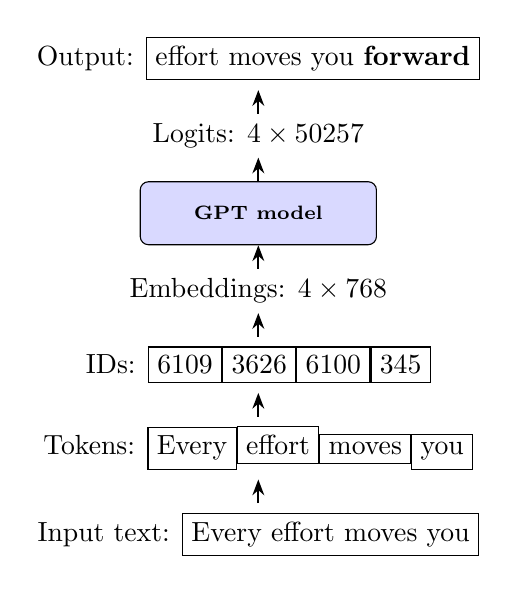
\begin{tikzpicture}[node distance=0.3cm]
				\node (txt) {Input text: \fbox{Every effort moves you}};
				\node[above=of txt] (tk) {Tokens: \fbox{Every}\fbox{effort}\fbox{moves}\fbox{you}};
				\node[above=of tk] (ids) {IDs: \fbox{6109}\fbox{3626}\fbox{6100}\fbox{345}};
				\node[above=of ids] (em) {Embeddings: $4\times768$};
				\node[box, fill=blue!15, minimum width=3cm, minimum height=0.8cm, above=of em] (gpt) {\textbf{GPT model}};
				\node[above=of gpt] (lo) {Logits: $4\times50257$};
				\node[above=of lo] (ot) {Output: \fbox{effort moves you \textbf{forward}}};
				\draw[arr] (txt) -- (tk); \draw[arr] (tk) -- (ids); \draw[arr] (ids) -- (em);
				\draw[arr] (em) -- (gpt); \draw[arr] (gpt) -- (lo); \draw[arr] (lo) -- (ot);
			\end{tikzpicture}
			\column{0.45\textwidth}
			\small
			\begin{itemize}
				\item Tokenize a batch of 2 texts with \texttt{tiktoken} (GPT-2 BPE).
				\item Input shape: \texttt{[2, 4]}
				\item Output shape: \texttt{[2, 4, 50257]}
				\item One \textbf{logit vector per token}, one dimension per vocabulary entry.
				\item The last row should predict the \textbf{next} word.
			\end{itemize}
		\end{columns}
	\end{frame}
	
	% =====================================================================
	\section{Layer normalization}
	% =====================================================================
	
	\begin{frame}{Why normalize?}
		\begin{itemize}
			\item Deep networks suffer from \textbf{vanishing / exploding gradients} $\Rightarrow$ unstable training.
			\item \textbf{Idea:} rescale the activations of a layer to \textbf{mean 0} and \textbf{variance 1}.
			\item Faster convergence and more reliable training.
		\end{itemize}
		\begin{equation*}
			\text{LayerNorm}(\mathbf{x}) = \gamma \odot \frac{\mathbf{x} - \mu}{\sqrt{\sigma^2 + \epsilon}} + \beta,
			\qquad
			\mu = \frac{1}{d}\sum_{i=1}^{d} x_i, \quad
			\sigma^2 = \frac{1}{d}\sum_{i=1}^{d} (x_i-\mu)^2
		\end{equation*}
		\begin{itemize}
			\item Computed over the \textbf{feature (embedding) dimension} of each token.
			\item $\gamma$ (\emph{scale}) and $\beta$ (\emph{shift}) are \textbf{trainable}.
			\item $\epsilon$ (e.g.\ $10^{-5}$) avoids division by zero.
		\end{itemize}
	\end{frame}
	
	\begin{frame}{Layer normalization: an example}
		\centering
		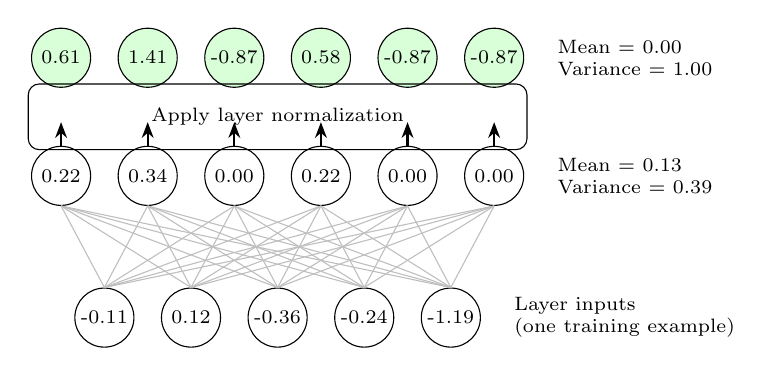
\begin{tikzpicture}[circ/.style={draw, circle, minimum size=0.75cm, font=\scriptsize, inner sep=0pt}]
			\foreach \v [count=\i] in {-0.11,0.12,-0.36,-0.24,-1.19}
			\node[circ] (i\i) at (\i*1.1+0.55, 0) {\v};
			\foreach \v [count=\i] in {0.22,0.34,0.00,0.22,0.00,0.00}
			\node[circ] (h\i) at (\i*1.1, 1.8) {\v};
			\foreach \v [count=\i] in {0.61,1.41,-0.87,0.58,-0.87,-0.87}
			\node[circ, fill=green!15] (o\i) at (\i*1.1, 3.3) {\v};
			\foreach \a in {1,...,5} \foreach \b in {1,...,6} \draw[gray!50] (i\a.north) -- (h\b.south);
			\node[draw, rounded corners, fit=(h1)(h6), inner sep=1pt, yshift=0.75cm, minimum height=0.35cm, font=\scriptsize, label={[font=\scriptsize]center:Apply layer normalization}] {};
			\foreach \b in {1,...,6} \draw[arr] (h\b.north) -- ++(0,0.3);
			\node[right=0.3cm of i5, font=\scriptsize, align=left] {Layer inputs\\(one training example)};
			\node[right=0.3cm of h6, font=\scriptsize, align=left] {Mean = 0.13\\Variance = 0.39};
			\node[right=0.3cm of o6, font=\scriptsize, align=left] {Mean = 0.00\\Variance = 1.00};
		\end{tikzpicture}
	\end{frame}
	
	\begin{frame}[fragile]{Computing mean and variance in PyTorch}
		\begin{columns}[T]
			\column{0.52\textwidth}
			\begin{lstlisting}
		torch.manual_seed(123)
		batch_example = torch.randn(2, 5)
		layer = nn.Sequential(nn.Linear(5, 6), nn.ReLU())
		out = layer(batch_example)				
		mean = out.mean(dim=-1, keepdim=True)
		var  = out.var(dim=-1, keepdim=True)
		out_norm = (out - mean) / torch.sqrt(var)
			\end{lstlisting}
			\footnotesize
			\texttt{keepdim=True} keeps a \texttt{[2,1]} shape instead of \texttt{[2]}, so broadcasting works.
			\column{0.46\textwidth}
			\begin{itemize}
				\footnotesize
				\item \texttt{dim=-1}: last dimension (one statistic \textbf{per row}).
				\item \texttt{dim=0}: one statistic \textbf{per column}.
				\item With 3D tensors \texttt{[batch, tokens, emb]}, \texttt{dim=-1} still normalizes each token's embedding.
			\end{itemize}
			\vspace{0.2cm}
			\scriptsize
			\begin{tabular}{lcc}
				\toprule
				& Mean & Variance \\
				\midrule
				Before & 0.1324 / 0.2170 & 0.0231 / 0.0398 \\
				After  & $\approx 0$ & 1.0 \\
				\bottomrule
			\end{tabular}
		\end{columns}
	\end{frame}
	
	\begin{frame}[fragile]{A \texttt{LayerNorm} module}
		\begin{lstlisting}
			class LayerNorm(nn.Module):
			def __init__(self, emb_dim):
			super().__init__()
			self.eps = 1e-5
			self.scale = nn.Parameter(torch.ones(emb_dim))   # gamma
			self.shift = nn.Parameter(torch.zeros(emb_dim))  # beta
			
			def forward(self, x):
			mean = x.mean(dim=-1, keepdim=True)
			var = x.var(dim=-1, keepdim=True, unbiased=False)
			norm_x = (x - mean) / torch.sqrt(var + self.eps)
			return self.scale * norm_x + self.shift
		\end{lstlisting}
		\begin{block}{Biased variance (\texttt{unbiased=False})}
			\footnotesize Divides by $n$ instead of $n-1$ (no Bessel's correction). Negligible for large $n$, and it matches GPT-2's original TensorFlow implementation $\Rightarrow$ compatible with pretrained weights.
		\end{block}
	\end{frame}
	
	\begin{frame}{Layer norm vs.\ batch norm}
		\begin{columns}[c]
			\column{0.5\textwidth}
			\centering
			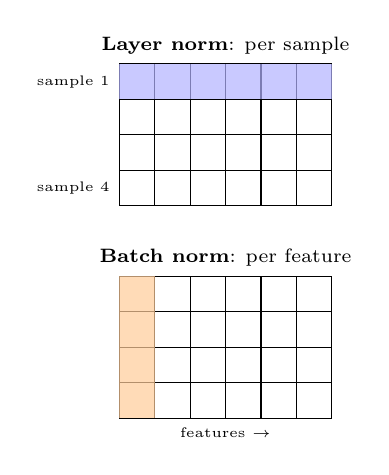
\begin{tikzpicture}[scale=0.45]
				\foreach \r in {0,...,3} \foreach \c in {0,...,5} \draw (\c,-\r) rectangle ++(1,1);
				\fill[blue!30, opacity=0.7] (0,0) rectangle (6,1);
				\node[font=\scriptsize, above] at (3,1) {\textbf{Layer norm}: per sample};
				\node[font=\tiny, left] at (0,0.5) {sample 1};
				\node[font=\tiny, left] at (0,-2.5) {sample 4};
				\begin{scope}[yshift=-6cm]
					\foreach \r in {0,...,3} \foreach \c in {0,...,5} \draw (\c,-\r) rectangle ++(1,1);
					\fill[orange!40, opacity=0.7] (0,-3) rectangle (1,1);
					\node[font=\scriptsize, above] at (3,1) {\textbf{Batch norm}: per feature};
					\node[font=\tiny, below] at (3,-3) {features $\rightarrow$};
				\end{scope}
			\end{tikzpicture}
			\column{0.5\textwidth}
			\begin{itemize}
				\item \textbf{Batch norm} normalizes across the \textbf{batch} dimension.
				\item \textbf{Layer norm} normalizes across the \textbf{feature} dimension.
				\item Layer norm is \textbf{independent of the batch size}:
				\begin{itemize}
					\item Works with batch size 1 at inference.
					\item Better for distributed training and constrained hardware.
				\end{itemize}
			\end{itemize}
		\end{columns}
	\end{frame}
	
	% =====================================================================
	\section{Feed forward network with GELU}
	% =====================================================================
	
	\begin{frame}{The GELU activation function}
		\begin{columns}[c]
			\column{0.45\textwidth}
			\small
			\begin{itemize}
				\item LLMs use smoother activations than ReLU: \textbf{GELU} and \textbf{SwiGLU}.
				\item Exact definition: $\text{GELU}(x) = x\,\Phi(x)$, with $\Phi$ the standard Gaussian CDF.
				\item GPT-2 uses the cheaper approximation:
			\end{itemize}
			\scriptsize
			\begin{equation*}
				\text{GELU}(x) \approx 0.5\,x\left(1 + \tanh\!\left[\sqrt{\tfrac{2}{\pi}}\left(x + 0.044715\,x^3\right)\right]\right)
			\end{equation*}
			\column{0.55\textwidth}
			\centering
			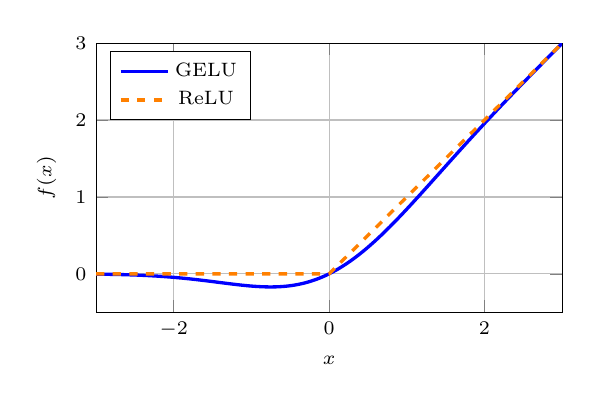
\begin{tikzpicture}
				\begin{axis}[
					width=7.5cm, height=5cm,
					xmin=-3, xmax=3, ymin=-0.5, ymax=3,
					grid=major, legend pos=north west,
					xlabel={$x$}, ylabel={$f(x)$},
					tick label style={font=\scriptsize}, label style={font=\scriptsize},
					legend style={font=\scriptsize}]
					\addplot[blue, very thick, domain=-3:3, samples=120]
					{0.5*x*(1+tanh(sqrt(2/pi)*(x+0.044715*x^3)))};
					\addlegendentry{GELU}
					\addplot[orange, very thick, dashed, domain=-3:3, samples=121]
					{max(0,x)};
					\addlegendentry{ReLU}
				\end{axis}
			\end{tikzpicture}
		\end{columns}
	\end{frame}
	
	\begin{frame}{GELU vs.\ ReLU}
		\begin{columns}[T]
			\column{0.5\textwidth}
			\textbf{ReLU}
			\begin{itemize}
				\item Piecewise linear: $\max(0,x)$.
				\item Sharp corner at 0 $\Rightarrow$ harder optimization in very deep networks.
				\item Zero output (and gradient) for every negative input.
			\end{itemize}
			\column{0.5\textwidth}
			\textbf{GELU}
			\begin{itemize}
				\item Smooth and non-linear everywhere.
				\item Allows more nuanced parameter updates.
				\item Small \textbf{non-zero} output for negative inputs $\Rightarrow$ those neurons still contribute to learning.
			\end{itemize}
		\end{columns}
	\end{frame}
	
	\begin{frame}[fragile]{The \texttt{FeedForward} module}
		\begin{columns}[c]
			\column{0.6\textwidth}
			\begin{lstlisting}[basicstyle=\ttfamily\tiny]
				class GELU(nn.Module):
				def forward(self, x):
				return 0.5 * x * (1 + torch.tanh(
				torch.sqrt(torch.tensor(2.0 / torch.pi)) *
				(x + 0.044715 * torch.pow(x, 3))))
				
				class FeedForward(nn.Module):
				def __init__(self, cfg):
				super().__init__()
				self.layers = nn.Sequential(
				nn.Linear(cfg["emb_dim"], 4 * cfg["emb_dim"]),
				GELU(),
				nn.Linear(4 * cfg["emb_dim"], cfg["emb_dim"]))
				
				def forward(self, x):
				return self.layers(x)
			\end{lstlisting}
			\column{0.38\textwidth}
			\centering
			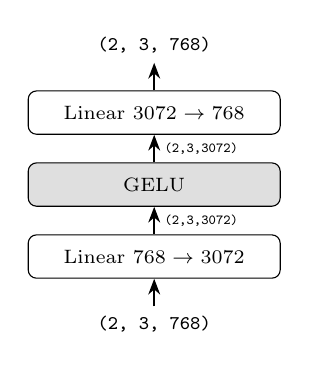
\begin{tikzpicture}[node distance=0.35cm]
				\node (in) {\scriptsize \texttt{(2, 3, 768)}};
				\node[box, above=of in] (l1) {Linear $768\to3072$};
				\node[fbox, above=of l1] (g) {GELU};
				\node[box, above=of g] (l2) {Linear $3072\to768$};
				\node[above=of l2] (out) {\scriptsize \texttt{(2, 3, 768)}};
				\draw[arr] (in) -- (l1); \draw[arr] (l1) -- node[right, font=\tiny]{\texttt{(2,3,3072)}} (g);
				\draw[arr] (g) -- node[right, font=\tiny]{\texttt{(2,3,3072)}} (l2); \draw[arr] (l2) -- (out);
			\end{tikzpicture}
		\end{columns}
	\end{frame}
	
	\begin{frame}{Expand, activate, contract}
		\begin{columns}[c]
			\column{0.5\textwidth}
			\centering
			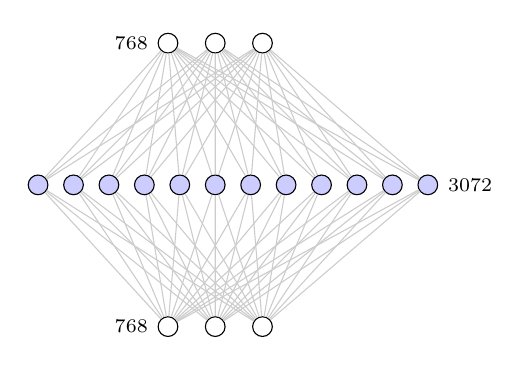
\begin{tikzpicture}[n/.style={draw, circle, minimum size=0.25cm, inner sep=0pt}]
				\foreach \i in {1,...,3} \node[n] (a\i) at (\i*0.6+1.2, 0) {};
				\foreach \i in {1,...,12} \node[n, fill=blue!20] (b\i) at (\i*0.45-0.3, 1.8) {};
				\foreach \i in {1,...,3} \node[n] (c\i) at (\i*0.6+1.2, 3.6) {};
				\foreach \i in {1,...,3} \foreach \j in {1,...,12} {\draw[gray!40] (a\i) -- (b\j); \draw[gray!40] (b\j) -- (c\i);}
				\node[font=\scriptsize, left] at (a1.west) {768};
				\node[font=\scriptsize, right] at (b12.east) {3072};
				\node[font=\scriptsize, left] at (c1.west) {768};
			\end{tikzpicture}
			\column{0.5\textwidth}
			\begin{itemize}
				\item First layer \textbf{expands} by a factor of 4 ($768\to3072$).
				\item GELU adds non-linearity in the larger space $\Rightarrow$ \textbf{richer representations}.
				\item Second layer \textbf{contracts} back to 768.
				\item Same input and output shape $\Rightarrow$ blocks can be \textbf{stacked} without adjusting dimensions.
				\item Works for any batch size and number of tokens.
			\end{itemize}
		\end{columns}
	\end{frame}
	
	% =====================================================================
	\section{Shortcut connections}
	% =====================================================================
	
	\begin{frame}{Shortcut (skip / residual) connections}
		\begin{columns}[c]
			\column{0.5\textwidth}
			\begin{itemize}
				\item Proposed in \textbf{ResNets} (computer vision) to fight \textbf{vanishing gradients}.
				\item Gradients shrink as they propagate backward $\Rightarrow$ early layers barely learn.
				\item A shortcut \textbf{adds the input of a layer to its output}:
			\end{itemize}
			\begin{equation*}
				\mathbf{x}_{\ell+1} = \mathbf{x}_\ell + f_\ell(\mathbf{x}_\ell)
			\end{equation*}
			\begin{itemize}
				\item Creates an alternative, shorter path for the gradient:
				$\frac{\partial \mathbf{x}_{\ell+1}}{\partial \mathbf{x}_\ell} = I + \frac{\partial f_\ell}{\partial \mathbf{x}_\ell}$
			\end{itemize}
			\column{0.45\textwidth}
			\centering
			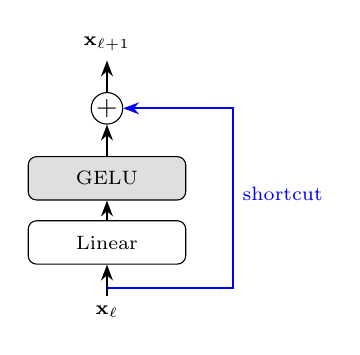
\begin{tikzpicture}[node distance=0.25cm]
				\node (x) {\scriptsize $\mathbf{x}_\ell$};
				\node[box, minimum width=2cm, above=0.4cm of x] (lin) {Linear};
				\node[fbox, minimum width=2cm, above=of lin] (g) {GELU};
				\node[draw, circle, inner sep=0pt, minimum size=0.4cm, above=0.4cm of g] (plus) {$+$};
				\node[above=0.4cm of plus] (y) {\scriptsize $\mathbf{x}_{\ell+1}$};
				\draw[arr] (x) -- (lin); \draw[arr] (lin) -- (g); \draw[arr] (g) -- (plus); \draw[arr] (plus) -- (y);
				\coordinate (split) at ($(x)!0.5!(lin.south)$);
				\draw[arr, blue, thick] (split) -- ++(1.6,0) |- (plus.east);
				\node[font=\scriptsize, blue, right] at ($(split)+(1.6,1.2)$) {shortcut};
			\end{tikzpicture}
		\end{columns}
	\end{frame}
	
	\begin{frame}[fragile]{Experiment: a 5-layer network with and without shortcuts}
		\begin{lstlisting}[basicstyle=\ttfamily\tiny]
			class ExampleDeepNeuralNetwork(nn.Module):
			def __init__(self, layer_sizes, use_shortcut):
			super().__init__()
			self.use_shortcut = use_shortcut
			self.layers = nn.ModuleList([
			nn.Sequential(nn.Linear(layer_sizes[i], layer_sizes[i+1]), GELU())
			for i in range(5)])
			
			def forward(self, x):
			for layer in self.layers:
			layer_output = layer(x)
			if self.use_shortcut and x.shape == layer_output.shape:
			x = x + layer_output       # shortcut connection
			else:
			x = layer_output
			return x
			
			layer_sizes  = [3, 3, 3, 3, 3, 1]
			sample_input = torch.tensor([[1., 0., -1.]])
		\end{lstlisting}
		\footnotesize We compute an MSE loss against target 0, call \texttt{loss.backward()} and print the \textbf{mean absolute gradient} of each layer's weights.
	\end{frame}
	
	\begin{frame}{Results: gradients per layer}
		\begin{columns}[c]
			\column{0.55\textwidth}
			\centering
			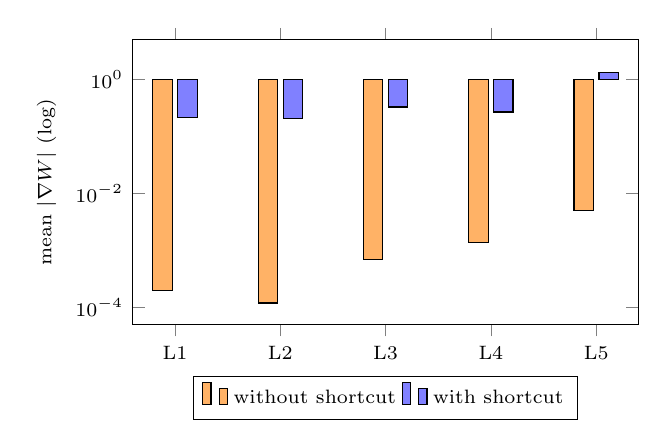
\begin{tikzpicture}
				\begin{axis}[
					ybar, bar width=7pt, width=8cm, height=5.2cm,
					ymode=log, ymin=5e-5, ymax=5,
					symbolic x coords={L1,L2,L3,L4,L5}, xtick=data,
					ylabel={mean $|\nabla W|$ (log)},
					legend style={font=\scriptsize, at={(0.5,-0.18)}, anchor=north, legend columns=2},
					tick label style={font=\scriptsize}, label style={font=\scriptsize}]
					\addplot[fill=orange!60] coordinates {(L1,0.0002) (L2,0.00012) (L3,0.0007) (L4,0.0014) (L5,0.0050)};
					\addplot[fill=blue!50] coordinates {(L1,0.22) (L2,0.21) (L3,0.33) (L4,0.27) (L5,1.33)};
					\legend{without shortcut, with shortcut}
				\end{axis}
			\end{tikzpicture}
			\column{0.45\textwidth}
			\small
			\begin{itemize}
				\item \textbf{Without} shortcuts: the gradient shrinks from $0.005$ (layer 5) to $0.0002$ (layer 1) $\Rightarrow$ \textbf{vanishing gradient}.
				\item \textbf{With} shortcuts: gradients stay around $0.2$--$0.3$ even in the first layers.
				\item Shortcuts are a \textbf{core building block} of LLMs: they keep gradient flow consistent across dozens of layers.
			\end{itemize}
		\end{columns}
	\end{frame}
	
	% =====================================================================
	\section{The transformer block}
	% =====================================================================
	
	\begin{frame}{Progress so far}
		\centering
		\roadmapfig{6}
		
		\vspace{0.3cm}
		\small Now we combine blocks 2--5 with multi-head attention into a \textbf{transformer block}.
	\end{frame}
	
	\begin{frame}{Anatomy of the transformer block}
		\begin{columns}[c]
			\column{0.42\textwidth}
			\centering
			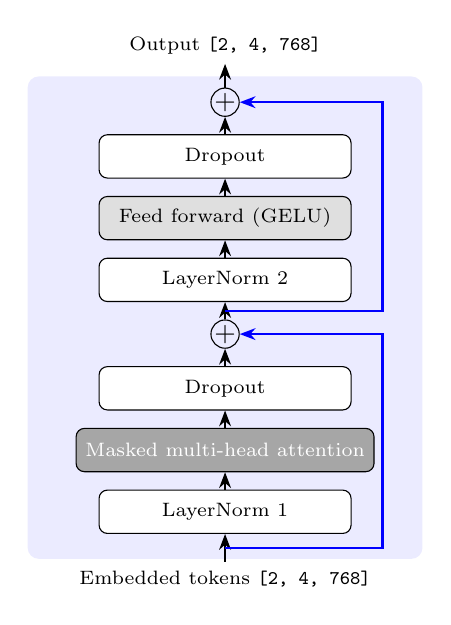
\begin{tikzpicture}[node distance=0.22cm]
				\node (in) {\scriptsize Embedded tokens \texttt{[2, 4, 768]}};
				\node[box, above=0.35cm of in] (n1) {LayerNorm 1};
				\node[dbox, above=of n1] (mha) {Masked multi-head attention};
				\node[box, above=of mha] (d1) {Dropout};
				\node[draw, circle, inner sep=0pt, minimum size=0.35cm, above=of d1] (p1) {$+$};
				\node[box, above=of p1] (n2) {LayerNorm 2};
				\node[fbox, above=of n2] (ff) {Feed forward (GELU)};
				\node[box, above=of ff] (d2) {Dropout};
				\node[draw, circle, inner sep=0pt, minimum size=0.35cm, above=of d2] (p2) {$+$};
				\node[above=0.3cm of p2] (out) {\scriptsize Output \texttt{[2, 4, 768]}};
				\draw[arr] (in) -- (n1); \draw[arr] (n1) -- (mha); \draw[arr] (mha) -- (d1); \draw[arr] (d1) -- (p1);
				\draw[arr] (p1) -- (n2); \draw[arr] (n2) -- (ff); \draw[arr] (ff) -- (d2); \draw[arr] (d2) -- (p2); \draw[arr] (p2) -- (out);
				\coordinate (s1) at ($(in.north)!0.5!(n1.south)$);
				\coordinate (s2) at ($(p1.north)!0.5!(n2.south)$);
				\draw[arr, blue] (s1) -- ++(2.0,0) |- (p1.east);
				\draw[arr, blue] (s2) -- ++(2.0,0) |- (p2.east);
				\begin{scope}[on background layer]
					\node[fill=blue!8, rounded corners, fit=(n1)(p2)(s1), inner xsep=0.9cm, inner ysep=4pt] {};
				\end{scope}
			\end{tikzpicture}
			\column{0.56\textwidth}
			\small
			\begin{itemize}
				\item \textbf{Self-attention} relates tokens \textbf{to each other}.
				\item \textbf{Feed forward} transforms each position \textbf{independently}.
				\item \textbf{Pre-LayerNorm}: normalize \emph{before} each sub-layer (GPT-2 and modern LLMs). The original Transformer used \emph{Post-LayerNorm}, with worse training dynamics.
				\item \textbf{Dropout} after each sub-layer for regularization.
				\item \textbf{Shortcut} around each sub-layer.
				\item Repeated \textbf{12 times} in GPT-2 small.
			\end{itemize}
		\end{columns}
	\end{frame}
	
	\begin{frame}[fragile]{\texttt{TransformerBlock} in code}
		\begin{columns}[T]
			\column{0.55\textwidth}
			\begin{lstlisting}[basicstyle=\ttfamily\tiny]
				class TransformerBlock(nn.Module):
				def __init__(self, cfg):
				super().__init__()
				self.att = MultiHeadAttention(
				d_in=cfg["emb_dim"],
				d_out=cfg["emb_dim"],
				block_size=cfg["context_length"],
				num_heads=cfg["n_heads"],
				dropout=cfg["drop_rate"],
				qkv_bias=cfg["qkv_bias"])
				self.ff = FeedForward(cfg)
				self.norm1 = LayerNorm(cfg["emb_dim"])
				self.norm2 = LayerNorm(cfg["emb_dim"])
				self.drop_resid = nn.Dropout(cfg["drop_rate"])
			\end{lstlisting}
			\column{0.43\textwidth}
			\begin{lstlisting}[basicstyle=\ttfamily\tiny]
				def forward(self, x):
				# Attention sub-layer
				shortcut = x
				x = self.norm1(x)
				x = self.att(x)
				x = self.drop_resid(x)
				x = x + shortcut
				
				# Feed forward sub-layer
				shortcut = x
				x = self.norm2(x)
				x = self.ff(x)
				x = self.drop_resid(x)
				x = x + shortcut
				return x
			\end{lstlisting}
		\end{columns}
	\end{frame}
	
	\begin{frame}{Shape preservation}
		\begin{itemize}
			\item Input \texttt{[2, 4, 768]} $\to$ output \texttt{[2, 4, 768]}.
			\item This is a \textbf{design decision}, not an accident:
			\begin{itemize}
				\item Blocks can be stacked freely.
				\item One output vector per input token (one-to-one).
			\end{itemize}
			\item The \textbf{shape} stays the same, but the \textbf{content} changes: each output is a \textbf{context vector} that integrates information from the whole (previous) sequence.
		\end{itemize}
		\begin{equation*}
			\underbrace{\mathbf{x}_1,\dots,\mathbf{x}_n}_{\text{token embeddings}}
			\;\xrightarrow{\text{Transformer block}}\;
			\underbrace{\mathbf{z}_1,\dots,\mathbf{z}_n}_{\text{context vectors}},
			\qquad \mathbf{x}_i,\mathbf{z}_i \in \mathbb{R}^{768}
		\end{equation*}
	\end{frame}
	
	% =====================================================================
	\section{Coding the GPT model}
	% =====================================================================
	
	\begin{frame}{The full GPT-2 architecture}
		\begin{columns}[c]
			\column{0.42\textwidth}
			\centering
			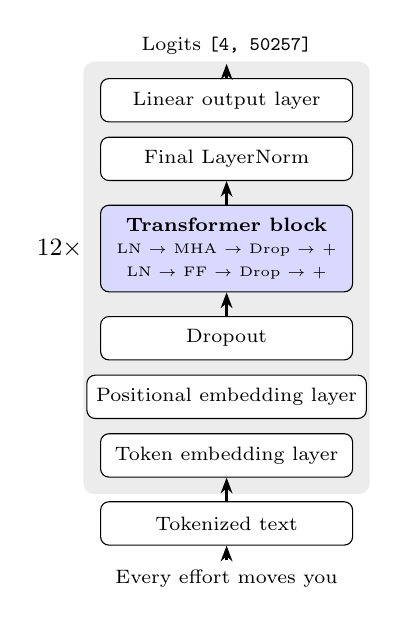
\begin{tikzpicture}[node distance=0.18cm]
				\node (in) {\scriptsize Every effort moves you};
				\node[box, above=of in] (tt) {Tokenized text};
				\node[box, above=0.3cm of tt] (te) {Token embedding layer};
				\node[box, above=of te] (pe) {Positional embedding layer};
				\node[box, above=of pe] (de) {Dropout};
				\node[box, fill=blue!15, minimum height=1.1cm, above=0.3cm of de] (tb) {\textbf{Transformer block}\\{\tiny LN $\to$ MHA $\to$ Drop $\to$ $+$}\\{\tiny LN $\to$ FF $\to$ Drop $\to$ $+$}};
				\node[box, above=0.3cm of tb] (fn) {Final LayerNorm};
				\node[box, above=of fn] (ol) {Linear output layer};
				\node[above=of ol] (lo) {\scriptsize Logits \texttt{[4, 50257]}};
				\draw[arr] (in) -- (tt); \draw[arr] (tt) -- (te); \draw[arr] (de) -- (tb); \draw[arr] (tb) -- (fn); \draw[arr] (ol) -- (lo);
				\node[left=0.1cm of tb, font=\small] {$12\times$};
				\begin{scope}[on background layer]
					\node[fill=gray!15, rounded corners, fit=(te)(ol), inner sep=6pt] {};
				\end{scope}
			\end{tikzpicture}
			\column{0.56\textwidth}
			\small
			\begin{enumerate}
				\item Token IDs $\to$ \textbf{token embeddings} + \textbf{positional embeddings}.
				\item Dropout on the embeddings.
				\item \textbf{12 stacked transformer blocks} (36 in GPT-2 XL\textsuperscript{*}).
				\item \textbf{Final LayerNorm}.
				\item \textbf{Linear output head}: $768 \to 50{,}257$ (vocabulary size) $\Rightarrow$ scores for the next token.
			\end{enumerate}
			\vspace{0.2cm}
			\scriptsize \textsuperscript{*}As stated in the book; the original GPT-2 XL has 48 layers (see Exercise 4.2).
		\end{columns}
	\end{frame}
	
	\begin{frame}[fragile]{\texttt{GPTModel} in code}
		\begin{lstlisting}[basicstyle=\ttfamily\tiny]
			class GPTModel(nn.Module):
			def __init__(self, cfg):
			super().__init__()
			self.tok_emb = nn.Embedding(cfg["vocab_size"], cfg["emb_dim"])
			self.pos_emb = nn.Embedding(cfg["context_length"], cfg["emb_dim"])
			self.drop_emb = nn.Dropout(cfg["drop_rate"])
			self.trf_blocks = nn.Sequential(
			*[TransformerBlock(cfg) for _ in range(cfg["n_layers"])])
			self.final_norm = LayerNorm(cfg["emb_dim"])
			self.out_head = nn.Linear(cfg["emb_dim"], cfg["vocab_size"], bias=False)
			
			def forward(self, in_idx):
			batch_size, seq_len = in_idx.shape
			tok_embeds = self.tok_emb(in_idx)
			pos_embeds = self.pos_emb(torch.arange(seq_len, device=in_idx.device))
			x = self.drop_emb(tok_embeds + pos_embeds)
			x = self.trf_blocks(x)
			x = self.final_norm(x)
			logits = self.out_head(x)
			return logits
		\end{lstlisting}
		\footnotesize Identical to \texttt{DummyGPTModel}, with the real \texttt{TransformerBlock} and \texttt{LayerNorm}.
	\end{frame}
	
	\begin{frame}[fragile]{How many parameters?}
		\begin{columns}[T]
			\column{0.55\textwidth}
			\begin{lstlisting}
				model = GPTModel(GPT_CONFIG_124M)
				total_params = sum(p.numel()
				for p in model.parameters())
				# Total number of parameters: 163,009,536
			\end{lstlisting}
			\small Why 163M and not 124M?
			\begin{itemize}
				\item \texttt{tok\_emb.weight}: \texttt{[50257, 768]}
				\item \texttt{out\_head.weight}: \texttt{[50257, 768]}
				\item $50{,}257 \times 768 = 38{,}597{,}376$ params each!
			\end{itemize}
			\column{0.43\textwidth}
			\begin{block}{Weight tying}
				\footnotesize The original GPT-2 \textbf{reuses the token embedding weights} in the output layer.
				\[
				163{,}009{,}536 - 38{,}597{,}376 = \mathbf{124{,}412{,}160}
				\]
			\end{block}
			\footnotesize
			\begin{itemize}
				\item Tying reduces memory and compute.
				\item Separate layers often train better; most modern LLMs do so.
				\item We revisit tying when loading OpenAI's weights.
			\end{itemize}
		\end{columns}
	\end{frame}
	
	\begin{frame}{Memory footprint}
		\begin{itemize}
			\item Each parameter is a 32-bit float = \textbf{4 bytes}.
		\end{itemize}
		\begin{equation*}
			\frac{163{,}009{,}536 \times 4 \text{ bytes}}{1024^2} \approx \mathbf{621.83\ MB}
		\end{equation*}
		\begin{itemize}
			\item Even a ``small'' LLM needs significant storage.
			\item By the same rule, a 175B-parameter model needs $\approx$ \textbf{700 GB} in FP32 (just for the weights).
			\item This motivates lower precision formats (FP16, BF16, INT8, \dots).
		\end{itemize}
	\end{frame}
	
	% =====================================================================
	\section{Generating text}
	% =====================================================================
	
	\begin{frame}{Generating one token at a time}
		\centering
		{\renewcommand{\arraystretch}{1.8}
			\begin{tabular}{r l}
				\scriptsize 1st iteration: & \tk{Hello}\tk{,}\tk{I}\tk{am}\nw{a} \\
				\scriptsize 2nd iteration: & \tk{Hello}\tk{,}\tk{I}\tk{am}\tk{a}\nw{model} \\
				\scriptsize 3rd iteration: & \tk{Hello}\tk{,}\tk{I}\tk{am}\tk{a}\tk{model}\nw{ready} \\
				$\vdots$ & \\
				\scriptsize 6th iteration: & \tk{Hello}\tk{,}\tk{I}\tk{am}\tk{a}\tk{model}\tk{ready}\tk{to}\tk{help}\nw{.} \\
		\end{tabular}}
		
		\vspace{0.4cm}
		\raggedright
		\small The predicted token is \textbf{appended} to the input; the context \textbf{grows} at each iteration (autoregressive generation).
	\end{frame}
	
	\begin{frame}{One generation step in detail}
		\begin{columns}[c]
			\column{0.55\textwidth}
			\centering
			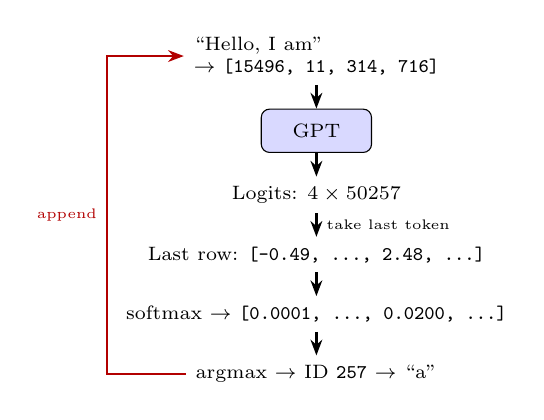
\begin{tikzpicture}[node distance=0.3cm, every node/.style={font=\scriptsize}]
				\node[align=left] (ids) {``Hello, I am''\\$\to$ \texttt{[15496, 11, 314, 716]}};
				\node[box, minimum width=1.4cm, fill=blue!15, below=of ids] (gpt) {GPT};
				\node[below=of gpt] (log) {Logits: $4 \times 50257$};
				\node[below=of log] (last) {Last row: \texttt{[-0.49, \dots, 2.48, \dots]}};
				\node[below=of last] (prob) {softmax $\to$ \texttt{[0.0001, \dots, 0.0200, \dots]}};
				\node[below=of prob] (arg) {argmax $\to$ ID \texttt{257} $\to$ ``a''};
				\draw[arr] (ids) -- (gpt); \draw[arr] (gpt) -- (log); \draw[arr] (log) -- node[right]{\tiny take last token} (last);
				\draw[arr] (last) -- (prob); \draw[arr] (prob) -- (arg);
				\draw[arr, red!70!black] (arg.west) -- ++(-1.0,0) |- node[pos=0.25, left]{\tiny append} (ids.west);
			\end{tikzpicture}
			\column{0.43\textwidth}
			\small
			\begin{enumerate}
				\item Encode text into token IDs.
				\item Run the model $\to$ logits.
				\item Keep the \textbf{last} vector (next-token prediction).
				\item Softmax $\to$ probabilities.
				\item Argmax $\to$ token ID.
				\item Append and repeat.
			\end{enumerate}
		\end{columns}
	\end{frame}
	
	\begin{frame}[fragile]{\texttt{generate\_text\_simple}}
		\begin{lstlisting}[basicstyle=\ttfamily\tiny]
			def generate_text_simple(model, idx, max_new_tokens, context_size):
			# idx: [batch, n_tokens] array of token IDs in the current context
			for _ in range(max_new_tokens):
			idx_cond = idx[:, -context_size:]          # crop to supported context
			with torch.no_grad():
			logits = model(idx_cond)               # [batch, n_tokens, vocab]
			logits = logits[:, -1, :]                  # only the last time step
			probas = torch.softmax(logits, dim=-1)     # [batch, vocab]
			idx_next = torch.argmax(probas, dim=-1, keepdim=True)  # [batch, 1]
			idx = torch.cat((idx, idx_next), dim=1)    # append
			return idx
		\end{lstlisting}
		\begin{itemize}
			\small
			\item Softmax is \textbf{monotonic}: argmax over logits gives the same result. Kept for intuition.
			\item Always choosing the most likely token = \textbf{greedy decoding}. Sampling strategies (temperature, top-$k$) come in the next chapter.
		\end{itemize}
	\end{frame}
	
	\begin{frame}[fragile]{Trying it out}
		\begin{lstlisting}[basicstyle=\ttfamily\tiny]
			start_context = "Hello, I am"
			encoded = tokenizer.encode(start_context)          # [15496, 11, 314, 716]
			encoded_tensor = torch.tensor(encoded).unsqueeze(0) # add batch dim -> [1, 4]
			
			model.eval()   # disable dropout
			out = generate_text_simple(model=model, idx=encoded_tensor,
			max_new_tokens=6,
			context_size=GPT_CONFIG_124M["context_length"])
			print(tokenizer.decode(out.squeeze(0).tolist()))
		\end{lstlisting}
		\begin{alertblock}{Output}
			\small \texttt{Hello, I am Featureiman Byeswickattribute argue logger Normandy \dots}
		\end{alertblock}
		\small Gibberish! The model has \textbf{random weights}: it has not been \textbf{trained} yet $\Rightarrow$ next chapter: pretraining.
	\end{frame}
	
	% =====================================================================
	\section{Summary and exercises}
	% =====================================================================
	
	\begin{frame}{Summary}
		\begin{itemize}
			\small
			\item \textbf{Layer normalization} stabilizes training by giving each layer's outputs a consistent mean and variance.
			\item \textbf{GELU} is a smooth activation used in the \textbf{feed forward} module (expand $\times4$, contract).
			\item \textbf{Shortcut connections} skip layers and mitigate vanishing gradients.
			\item \textbf{Transformer blocks} combine masked multi-head attention and feed forward networks with Pre-LayerNorm, dropout and shortcuts.
			\item \textbf{GPT models} stack many identical transformer blocks; the same \texttt{GPTModel} class covers 124M to 1.5B parameters.
			\item \textbf{Text generation} decodes the output one token at a time; without training the output is incoherent.
		\end{itemize}
	\end{frame}
	
	
	\begin{frame}[standout]
		Practice: Implementing a GPT model
	\end{frame}
	
\end{document}
